%%%%%%%%%%%%%%%%%%%%%%%%%%%%%%%%%%%%%%%%%
% University Assignment Title Page
% LaTeX Template
% Version 1.0 (27/12/12)
%
% This template has been downloaded from:
% http://www.LaTeXTemplates.com
%
% Original author:
% WikiBooks (http://en.wikibooks.org/wiki/LaTeX/Title_Creation)
%
% License:
% CC BY-NC-SA 3.0 (http://creativecommons.org/licenses/by-nc-sa/3.0/)
%
% Instructions for using this template:
% This title page is capable of being compiled as is. This is not useful for
% including it in another document. To do this, you have two options:
%
% 1) Copy/paste everything between \begin{document} and \end{document}
% starting at \begin{titlepage} and paste this into another LaTeX file where you
% want your title page.
% OR
% 2) Remove everything outside the \begin{titlepage} and \end{titlepage} and
% move this file to the same directory as the LaTeX file you wish to add it to.
% Then add \input{./title_page_1.tex} to your LaTeX file where you want your
% title page.
%
%%%%%%%%%%%%%%%%%%%%%%%%%%%%%%%%%%%%%%%%%
%\title{Title page with logo}
%----------------------------------------------------------------------------------------
%	PACKAGES AND OTHER DOCUMENT CONFIGURATIONS
%----------------------------------------------------------------------------------------

\documentclass[12pt]{article}

%encoding
%--------------------------------------
\usepackage[utf8]{inputenc}
\usepackage[T1]{fontenc}
%--------------------------------------

%--------------------------------------
\usepackage[english]{babel}
%--------------------------------------

% Enables side captions
\usepackage[rightcaption]{sidecap}

% Inline quotations
\usepackage{csquotes}

\usepackage{graphicx}

% Text highlighting
\usepackage{color,soul}
\usepackage{xcolor}

\definecolor{weirdblue}{RGB}{166, 200, 219}
\sethlcolor{weirdblue}

% Allows references
\usepackage{hyperref}

\hypersetup{
    colorlinks,
    citecolor=black,
    filecolor=black,
    linkcolor=black,
    urlcolor=black
}

% Fancy image borders
\usepackage[most]{tcolorbox}


\begin{document}
\begin{titlepage}

\newcommand{\HRule}{\rule{\linewidth}{0.5mm}} % Defines a new command for the horizontal lines, change thickness here

\center % Center everything on the page

%----------------------------------------------------------------------------------------
%	HEADING SECTIONS
%----------------------------------------------------------------------------------------

{ \huge \bfseries A crowdbook by \vspace{1cm}}\\[4.5cm] % Name of your university/college

%----------------------------------------------------------------------------------------
%	TITLE SECTION
%----------------------------------------------------------------------------------------

\HRule \\[1.5cm]\textsc{\LARGE Ants \& Ant Keeping}\\[0.4cm]\textsc{discord}\\[1.5cm] % Title of your document
\HRule

%----------------------------------------------------------------------------------------
%	AUTHOR SECTION
%----------------------------------------------------------------------------------------



%----------------------------------------------------------------------------------------
%	DATE SECTION
%----------------------------------------------------------------------------------------


%----------------------------------------------------------------------------------------
%	LOGO SECTION
%----------------------------------------------------------------------------------------


%----------------------------------------------------------------------------------------

\vfill % Fill the rest of the page with whitespace
\end{titlepage}
\newpage

\tableofcontents{}

\newpage
\listoffigures
\newpage

\section{Observations}

% ------------------------------------
% --- TEMPLATE FOR AN OBSERVATION  ---

% use SCfigure in order to side-caption the figure
\begin{SCfigure}[0.5][h]

% the label shall be the same as the file preceded by fig if it's labelling a figure
\label{fig:Noebl1[MA]-5-4-2019}

% use tcbox for a fancy border
% the filename of the picture shall be the name of the poster + the month and year
\tcbox{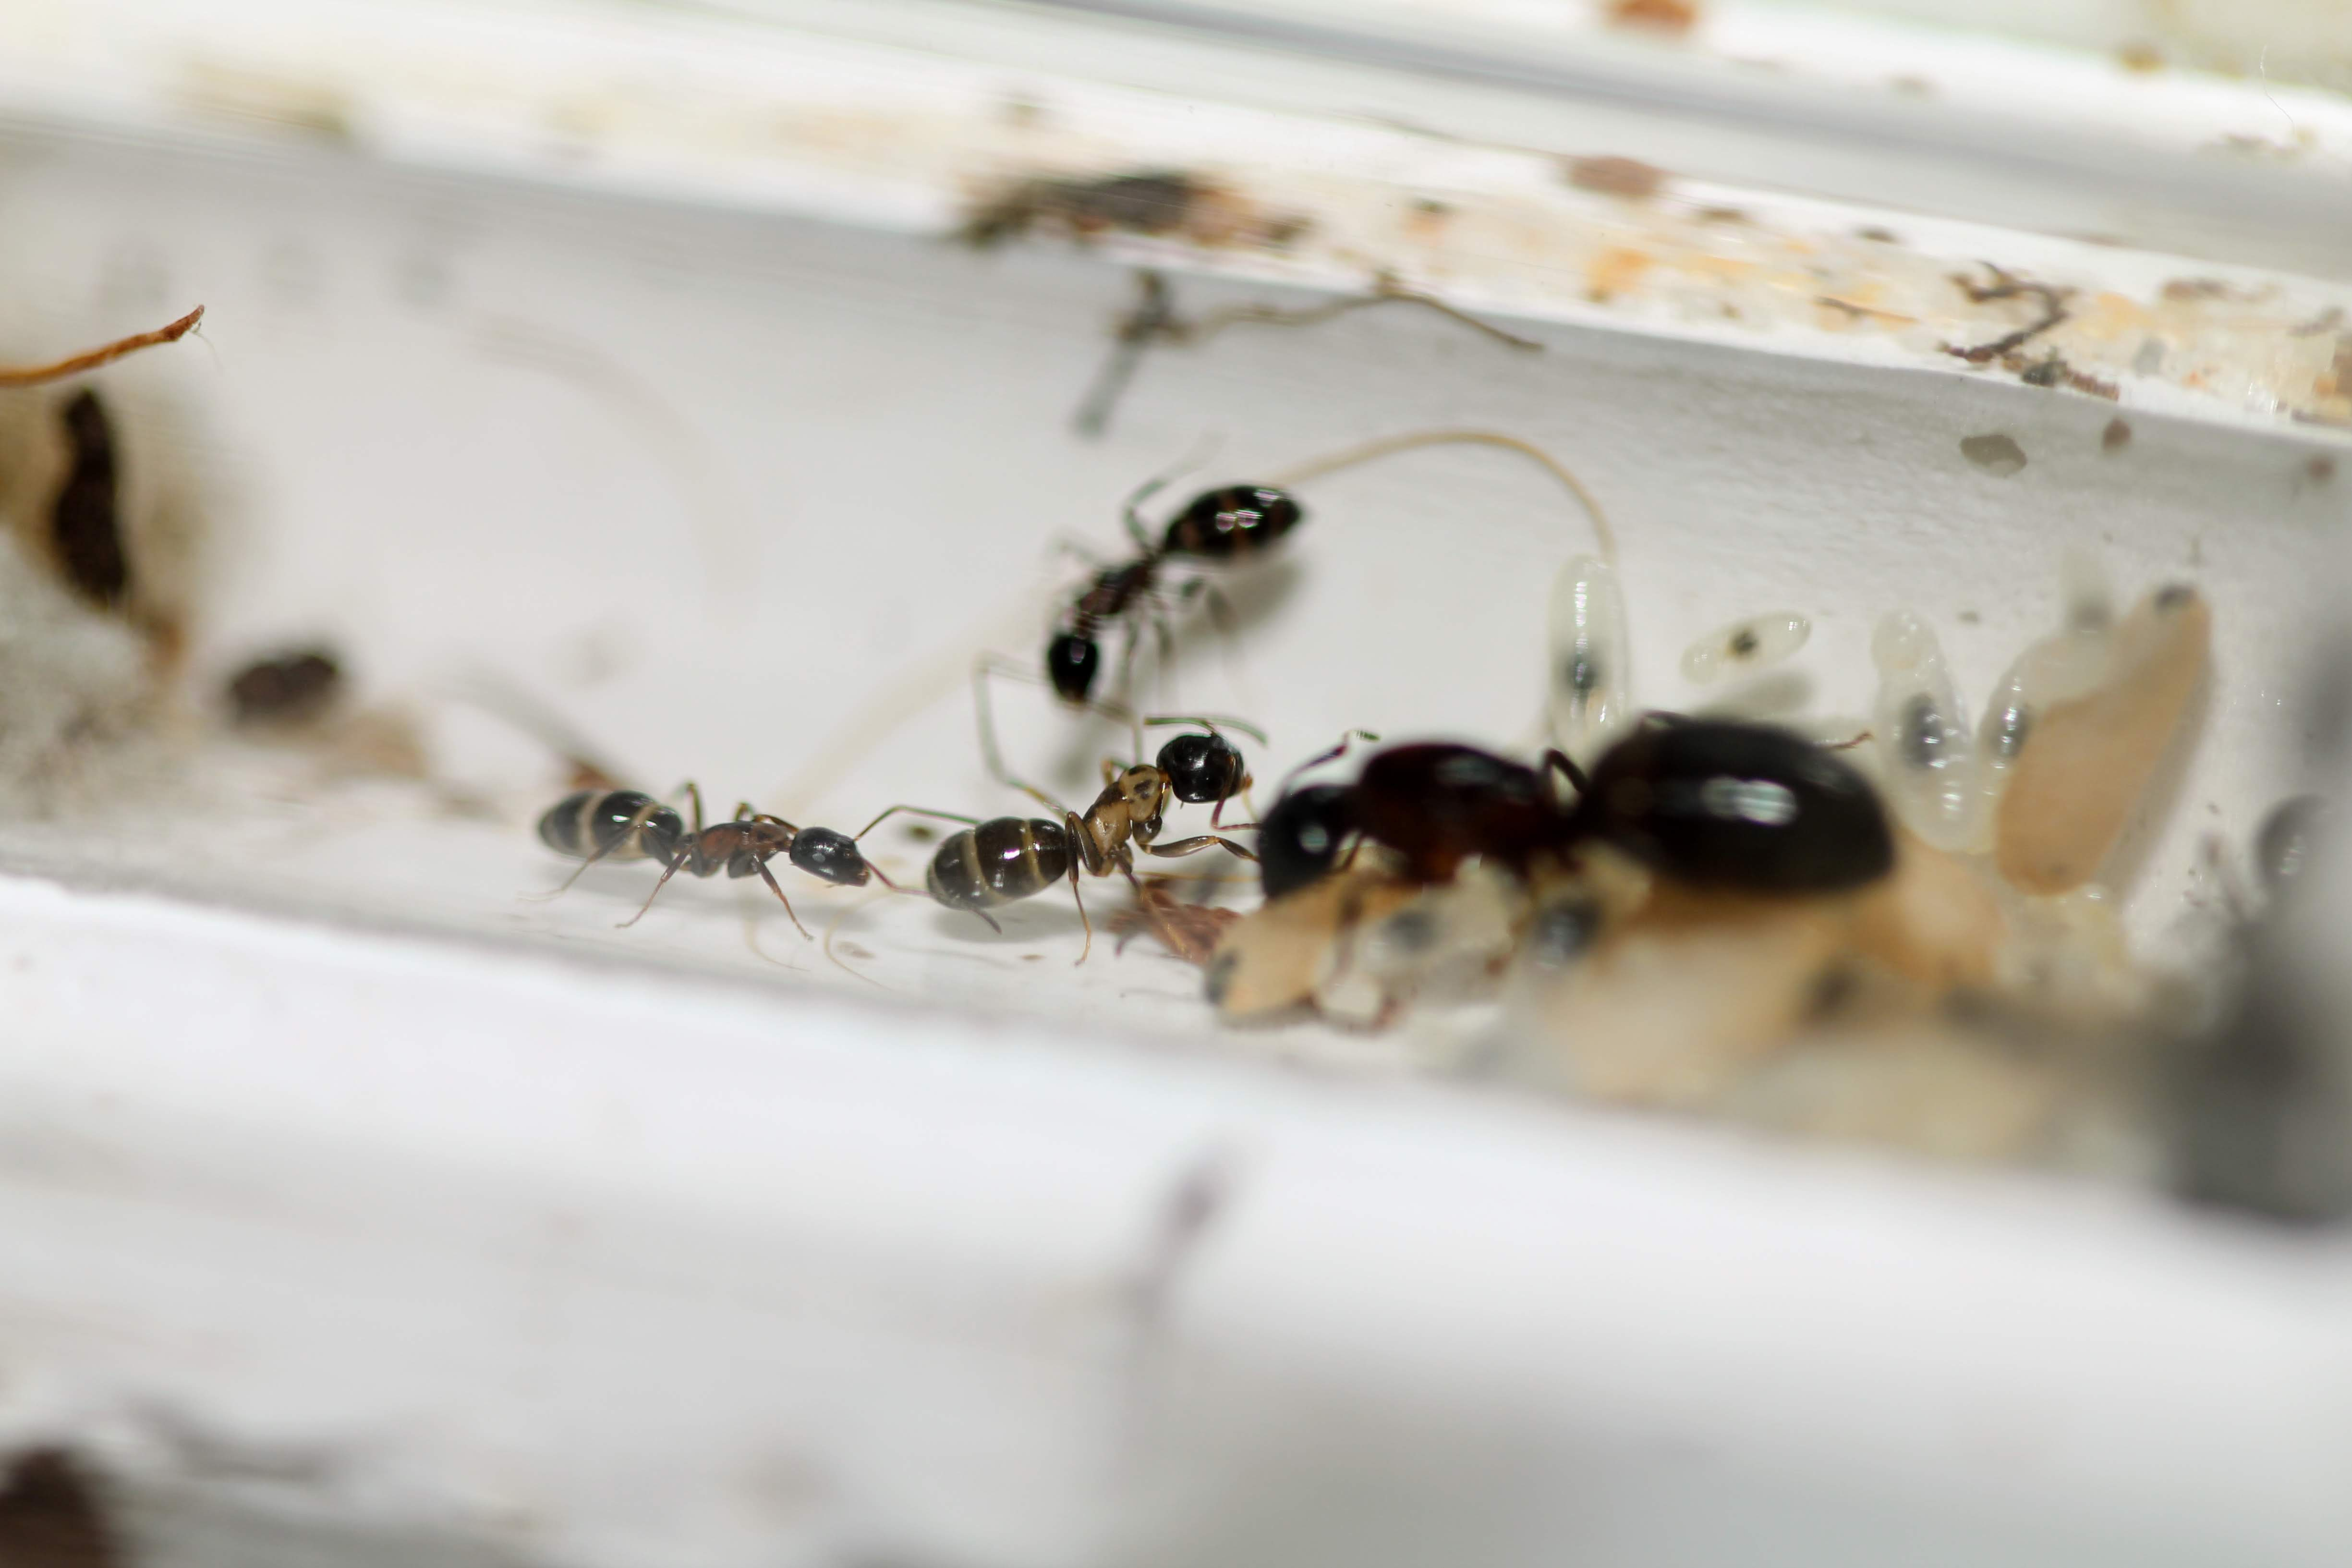
\includegraphics[width=0.6\textwidth]{ant_pictures/Noebl1[MA]-4-2019}}

% try to follow the same caption style
\caption{\textit{Camponotus Nearcticus}}
\end{SCfigure}

% \textsc has to precede \ul
\noindent\textsc{\ul{Noebl1[MA]}}:

% displayquote indents the text as desired
\begin{displayquote}
  48-hour-old first non-nanitic worker of the colony.
  \\Color still developing.
  \\The queen is the size of the average normal \textit Camponotus worker, so maybe 9-10mm.
\end{displayquote}

% ---      END OF TEMPLATE         ---
% ------------------------------------

\section{Cleaning Crews}
\section{[F]AQ.}

% ------------------------------------
% --- TEMPLATE FOR A QUESTION      ---

\subsection{If I freeze insects to feed ants, for how long would they remain edible?}

\noindent\textsc{\ul{Sirjordancurtis (CA)}}:

% Feel free to paraphrase/correct mistakes in the answer/question and
% please add the user who asked the question like so:
\begin{displayquote}
  \hl{@Grandma Yngvi}, you wouldn't want to use them after a few months because they start to freezer burn.
  \\At least that's true for birds, though I imagine it would also be unhealthy to feed extremely old crickets and mealworms to your ants
\end{displayquote}

% ---      END OF TEMPLATE         ---
% ------------------------------------

\subsection{How can I tell if it's an egg or small larva?}

\noindent\textsc{\ul{\#Infinity Vexation (OH)}}:

\begin{displayquote}
  \hl{@TugaNid (Portugal)}, a new larva looks just like an egg but bent.
  \\They usually only move when being fed.
\end{displayquote}

\begin{SCfigure}[0.5][h]

% the label shall be the same as the file preceded by fig if it's labelling a figure
\label{fig:ant-life-stages}

% use tcbox for a fancy border
% the filename of the picture shall be the name of the poster + the month and year
\tcbox{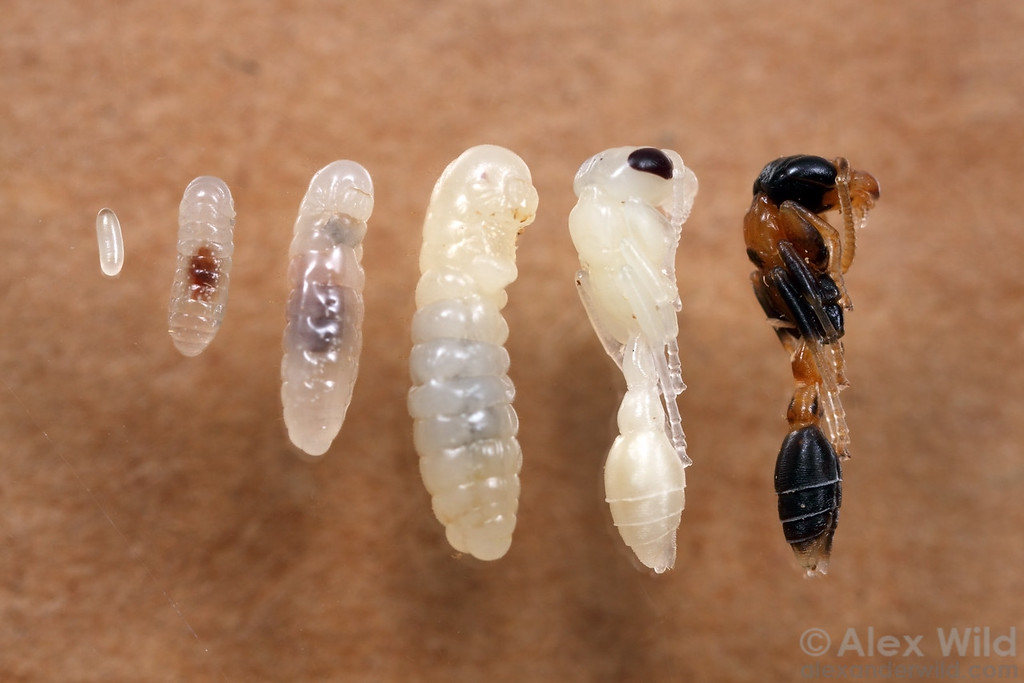
\includegraphics[width=0.6\textwidth]{ant_pictures/ant-life-stages}}

\caption{\textit{Side by side comparison of an ant's life stages}}
\end{SCfigure}

\end{document}
